
\section{Motivation} \label{sec:motivation}

%This section motivates for a more powerful function-merging technique with
%examples that highlight some of the weaknesses of the existing solutions, while
%also demonstrating how our optimization is able to overcome them.
%These examples contain real functions, extracted from the SPEC CPU2006 benchmark
%suite, that were carefully selected to show two distinct scenarios.
%The proposed optimization is the \textit{first} technique able to merge the
%functions shown in these examples.
%Note that, although we present the examples at the source level, the
%optimizations are actually implemented at the IR level.

As a motivation, consider two SPEC CPU2006 benchmark examples shown in Figures~\ref{fig:sphinx-example} and \ref{fig:libquantum-example}.

\begin{figure}[t!]
  \centering
  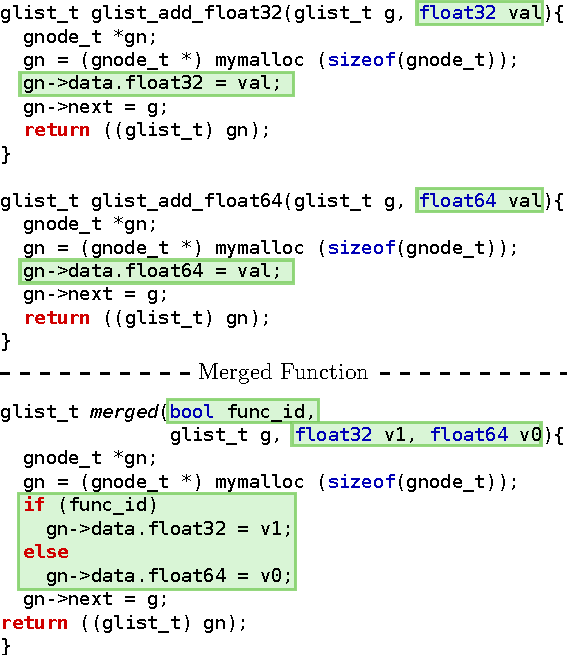
\includegraphics[width=.95\linewidth]{figs/sphinx-example.pdf}
  \caption{Example of two functions with different parameters that could be merged, as shown at the bottom.
           We highlight where they differ.}
  \label{fig:sphinx-example}
\end{figure}

Figure~\ref{fig:sphinx-example} shows two functions from the \texttt{482.sphinx3}. Although these two functions seem identical, their
function arguments are of different types, namely, \textit{float32} and \textit{float64}. In the diagram, we highlight the segments where
the data operations differ from each other. None of the the existing function-merging techniques would merge these two functions, as they
all require both functions to have exactly the same list of parameters, with the same types and in the same order. As shown at the bottom
of Figure~\ref{fig:sphinx-example}, these functions can be merged using two strategies. Firstly, we can expand the function argument list
to include the two parameters of different types. Then, we use a function identifier, \texttt{func\_id}, to indicate which of the two
functions is called. Function merging reduces the total number of machine instructions of the two functions by 18\%.

%If we compile all three functions, we can see that the each one of the two original functions have 14 machine instructions, while the merged function has 23 machine instructions.
%This represents a reduction of 18\% in the total number of instructions.
%However, the proposed optimization is able to merge them as shown at the bottom of Figure~\ref{fig:sphinx-example}. First, we merge both lists of parameters,
%adding an extra parameter used as an identifier to distinguish between the functions. Then, we guard the execution of the instructions that
%are unique to one of the functions using the function identifier. \fixme{ZW: Perhaps not talking about our technique here, but how much
%code reduction we can have by merging these two functions. We then use this to motivate the need of our technique.}

\begin{figure}[t!]
  \centering
  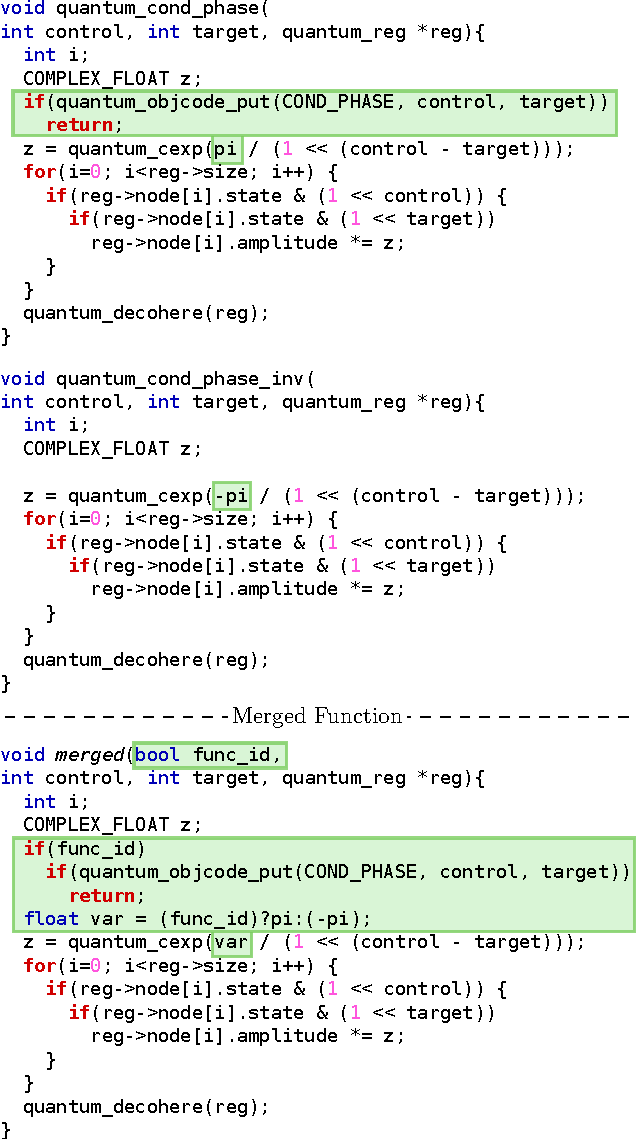
\includegraphics[width=\linewidth]{figs/libquantum-example.pdf}
  \caption{Example of two functions with different CFGs that could be merged, as shown at the bottom.
           We highlight where they differ.}
  \label{fig:libquantum-example}
\end{figure}


Figure~\ref{fig:libquantum-example} gives another two functions extracted from \texttt{462.libquantum}. Although these two functions have
the same signature, i.e., the same return type and list of parameters, they differ in some parts, including their CFGs. None of the
existing techniques can merge the two functions because of the difference in the CFGs. As shown at the bottom of
Figure~\ref{fig:libquantum-example}, these two functions in fact can be merged by simply using a function identifier, \texttt{func\_id}.
Function merging reduces the total number of machine instructions of the two functions by 23\%.

%The existing techniques are unable to merge them due mainly to the structural differences in their CFGs, as we have described in
%Section~\ref{sec:background}. Similar to the previous example, we could merge these two functions, as shown at the bottom of
%Figure~\ref{fig:libquantum-example}. Again, this can be done by using a function identifier. Inspecting the compiled assembly of all three
%functions, we can see a reduction of 27\% in the total number of machine instructions.
%%Similar to the previous example, the proposed optimization is also able to merge these two
%%functions, as shown at the bottom of Figure~\ref{fig:libquantum-example}. Basically, we guard the execution of the code that are unique to
%%one of the functions using the function identifier added to the list of parameters. \fixme{ZW: Again, here we need to give the intuition on
%%why we can merge them and what's the benefit for doing so. I think we should avoid talking about our technique here because at this point
%%the reviewer won't understand how our technique works.}
%=======
%Figure~\ref{fig:libquantum-example} shows two complete functions extracted from the SPEC CPU2006 \texttt{462.libquantum} benchmark.
%Although these two functions have the same signature, i.e., the same return type and list of parameters, they differ in some parts,
%including their CFGs. The existing techniques are unable to merge them due mainly to the structural differences in their CFGs, as we have
%described in Section~\ref{sec:background}.
%Similar to the previous example, we could merge these two functions, as shown at the bottom of Figure~\ref{fig:libquantum-example}. Basically, we just need to guard the execution of the code that is unique to
%one of the functions using the function identifier added to the list of parameters.
%Inspecting the compiled assembly of all three functions, we can see a reduction of 27\% in the total number of machine instructions.
%%Similar to the previous example, the proposed optimization is also able to merge these two
%%functions, as shown at the bottom of Figure~\ref{fig:libquantum-example}. Basically, we guard the execution of the code that are unique to
%%one of the functions using the function identifier added to the list of parameters. \fixme{ZW: Again, here we need to give the intuition on
%%why we can merge them and what's the benefit for doing so. I think we should avoid talking about our technique here because at this point
%%the reviewer won't understand how our technique works.}
%>>>>>>> e85b1a68ed569a46dd18b4379769346de63fc8f8


These examples show that the state-of-the-art function merging methods impose over-restricted constraints on the code structures, and thus
miss massive opportunities. Our work aims to develop a better approach to lift the constraints to merge similar code of any two arbitrary
functions.
